\section{Durchführung}
\label{sec:Durchführung}

\begin{figure}[H]
  \centering
  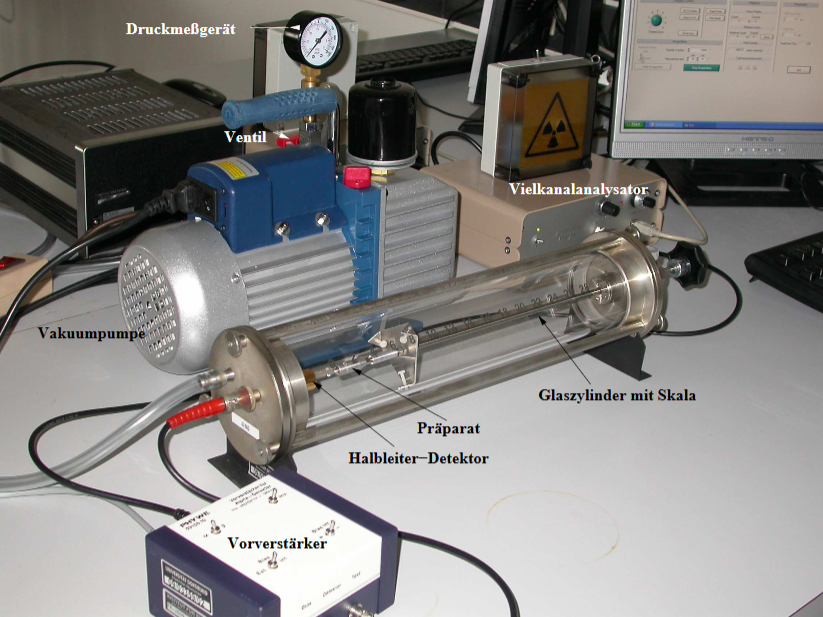
\includegraphics[height=8cm]{Aufbau.PNG}
  \caption{Aufbau der Messapparatur \cite{sample}.}
  \label{fig:aufbau}
\end{figure}

In Abbildung \ref{fig:aufbau} ist der Aufbau der verwendeten Messapparatur zu erkennen.
In einem Glaszylinder befindet sich eine Strahlungsquelle ($\alpha$-Strahlung) auf einer
beweglichen Schiene. Sie ist dabei in Richtung eines Halbleiter-Sperrschichtzählers am Ende
des Zylinders ausgerichtet. Dieser Zähler ist wiederum über einen Verstärker mit einem
Computer verbunden, auf welchem die gemessenen Zählraten graphisch dargestellt werden können.
Aus dem Glaszylinder kann dann noch die Luft mithilfe einer Vakuumpumpe evakuiert werden.

Zu Beginn des Versuchs wird die Strahlungsquelle bei normalem Luftdurch im Zylinder so weit
von dem Zähler entfernt, dass dieser gerade eben noch eine Strahlung misst. Außerdem wird
der Verstärker so angepasst, dass die gemessenen Zählraten trotz vorherrschendem Rauschen auf
dem Bildschirm des Computers gut sichtbar gemeacht werden können. Sodann wird
der Zylinder evakuiert. Anschließend wird Stück für Stück wieder Luft hinein gelassen.
Dabei werden jeweils bei unterschiedlichen Drücken (0-1000 mbar in 50 mbar Schritten)
über einen Zeitraum von 2 Minuten die Zählraten gemessen.
Danach wird eine analoge Messung mit einem leicht verringerten Abstand der Strahlungsquelle
zum Zähler durchgeführt.

Zum Schluss wird die Statistik des radioaktiven Zerfalls überprüft. Dafür wird der
Glaszylinder komplett evakuiert und die Strahlungsquelle wird verhältnismäßig weit vom
Zähler entfernt. Nun wird 100 mal über einen Zeitraum von jeweils zehn Sekunden die
Zählrate gemessen und die entsprechenden Wert vom Computer abgelesen.
